\chapter{Mechanizmy mediacji wiedzy}
\label{cha:mechanizmyMediacjiWiedzy}

%---------------------------------------------------------------------------

\section{Obszary zastosowań}
\label{sec:obszaryZastosowan}

Kluczowymi zastosowaniami mechanizmów mediacji wiedzy są te powiązane z~rozpoznawaniem emocji. Przede wszystkim chodzi tu o systemy rekomendacji, które najbardziej mogą skorzystać na dodatkowym rodzaju danych wejściowych, jakimi są emocje użytkownika. 

Wyobraźmy sobie system rekomendacji muzyki dużej aplikacji takiej jak Spotify. Dzięki dodatkowej wiedzy, mógłby zaproponować nam muzykę adekwatną do naszego nastroju. Podobnie sprawa ma się z~serwisami filmowymi takimi jak Netfix czy YouTube. Takie serwisy poza wyszukiwarką dysponują też stroną główną, na której przedstawiają użytkownikowi jak najlepsze propozycje. Wykorzystując informacje o naszych emocjach, te propozycje mogłyby być jeszcze lepsze. Kolejne możliwości pojawiają się w~obszarze zakupów. Platformy sprzedawcze takie jak Amazon czy Allegro mogłyby skorzystać z~efektów mediacji wiedzy proponując bardziej adekwatne produkty. Idąc dalej, przeglądarki internetowe takie jak Google czy DuckDuckGo mogłyby wyświetlać coraz lepsze propozycje.

Innym obszarem, gdzie mogłaby znaleźć zastosowanie wiedza zdobyta dzięki mechanizmom mediacji, mogłyby być gry i materiały edukacyjne. Emocje są niezwykle ważnym elementem przeżywania gier komputerowych. Znając reakcję gracza, system mógłby lepiej dostosować otaczający go świat.

%---------------------------------------------------------------------------

\section{Jawne metody mediacji wiedzy}
\label{sec:jawneMetodyMediacjiWiedzy}

Pierwszą z~kategorii metod mediacji wiedzy są metody jawne. Oznacza to, że w~proces mediacji zaangażowany jest sam użytkownik. To rozwiązanie ma swoje wady i zalety. Z pewnością największą zaletą jest skuteczność rozwiązania -- nikt nie wie więcej o stanie emocji niż sam użytkownik. Z kolei główną wadą jest fakt, że takie badanie może okazać się uciążliwe i irytujące, a na dłuższą metę zbytnio ingerujące w~życie człowieka, czy wręcz niemożliwe.

Przykładem jawnej metody może być praca Emilii Pieczonki realizowana na Katedrze Informatyki Stosowanej. W badaniach, jakie przeprowadziła, ''grupa użytkowników korzystajaca z~telefonu Android i aplikacji mobilnej, używała podczas codziennych czynności urządzenia sensorycznego na swoim nadgarstku i odpowiadała na pytania dotyczące ich samopoczucia'' \cite{EmiliaPieczonka}.

Warto również zwrócić uwagę na pracę Arkadiusza Lisa, również na Katedrze Informatyki Stosowanej. W tej pracy zostało wybrane w~oparciu o literaturę naukową kilka najbardziej obiecujących sposobów mediacji wiedzy. Następnie zaimplementowano zestaw widgetów, z~pomocą których użytkownik ''powinien być w~stanie subiektywnie określić stan emocjonalny (...), a następnie przekazać tą informację do systemu'' \cite{ArkadiuszLis}.

W pracy opisanej w~artykule \cite{hung2016predicting} naukowcy we współpracy z~psychiatrą stworzyli system, z~którego pomocą badany z~wykorzystaniem kolorowego suwaka może określić poziom swojego niepokoju czy gniewu. Badacze skupili się przede wszystkim nie na sensorach, ale na wzorcach korzystania z~telefonu udostępniach przez system operacyjnych takich jak wykonywanie połączeń, pisanie SMSów czy lokalizacja.

Mediacja nie musi odbywać się z~wykorzystaniem ekranu. Na rynku pojawiają się rozwiązania, w~których system głosowy taki jak Alexa, Asystent Google, Cortana czy Siri podczas rozmowy sam wypytuje użytkownika o nastrój.


%---------------------------------------------------------------------------

\section{Niejawne metody mediacji wiedzy}
\label{sec:niejawneMetodyMediacjiWiedzy}

Drugą kategorią metod mediacji wiedzy są metody niejawne. De facto sprowdza się to do braku bezpośredniego uczestnictwa człowieka w~przekazywaniu wiedzy. Oczywiście człowiek jest zaangażowany w~proces na przykład poprzez wykonywanie różnych czynności, ale nie zostanie nigdy zapytany wprost. Podobnie jak pierwsza kategoria, ta druga również ma swoje wady i zalety. Do zalet można zaliczyć wygodę -- korzystanie z~tych metod jest nieinwazyjne, nie ingeruje w~codzienną egzystencję. Minusem jest oczywiście mniejsza skuteczność.

Przykładem takiej mediacji może być praca \cite{zhang2011feature}, w~której naukowcy podejmują próby rozpoznania aktywności człowieka wykorzystując czujniki multimodalne. Do przetworzenia danych wykorzystywane są algorytmy wyboru cech.

Podobną metodą wykorzystali naukowcy w~pracy \cite{dai2010mobile} wykorzystując stworzony przez siebie model matematyczny w~celu określenia czy kierowca samochodu jest trzeźwy czy pijany.


%---------------------------------------------------------------------------

\section{Pozyskiwanie wiedzy o stanie emocjonalnym w~systemach \textit{affective computing}}
\label{sec:pozyskiwanieWiedzyOStanieEmocjonalnymWSystemachAffectiveComputing}

\textit{Affective computing} jest paradygmatem zaproponowanym przez Rosalind Picard z~Laboratorium Mediów MIT w~1997 roku\cite{picard1997affective}.

Wykorzystuje on rezultaty inżynierii biomedycznej, psychologii i sztucznej inteligencji. Celem jest pozwolenie systemom komputerowym wykrywać, wykorzystywać, a nawet wyrażać emocje\cite{nalepa2017affective}.

Przykładem pozyskiwania wiedzy może być gra wideo \textit{Bridge Scroll-runner} stworzona w~ramach pracy \cite{nalepa2017affective}. Naukowcy rozszerzyli możliwości gry wykorzystując czujniki tętna, temperatury skóry oraz reakcji galwanicznej skóry.

Rosaling Picard w~swojej pionierskiej pracy \cite{picard1997affective} jako przykład podaje komputerowy system uczący gry na pianinie. Taki system mógłby być znacznie skuteczniejszy od klasycznego systemu dysponując możliwością wyczuwania zainteresowania, przyjemności i smutku.

\begin{figure}[H]
	\centering
	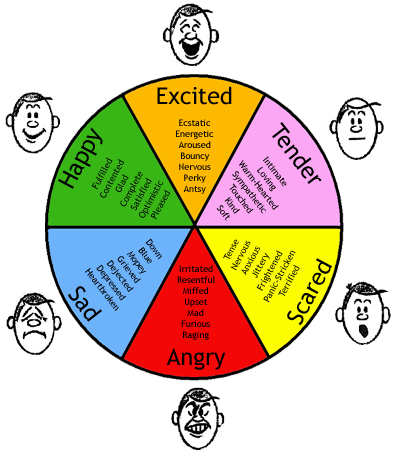
\includegraphics[scale=1]{rozdzial2/ModelEkmana.png}
	\caption{Koło podstawowych emocji (szczęście, podekscytowanie, rozczulenie, strach, gniew i smutek) i ich mimicznych ekspresji.}
\end{figure}

W niniejszej pracy zastosowano zarówno metody jawne jak i niejawne. W celu pozyskania wiedzy o stanie emocjonalnym zdecydowano się na syntezę odpowiedzi użytkownika i działania automatycznego systemu. Odpowiedzi użytkownika mogą być realizowane wprost poprzez aktywność z~listą emocji (jak na powyższym diagramie) i emotikon do wyboru lub (bardziej psychologicznie) z~wykorzystaniem palety kolorów. Automatyczny system wykorzystuje zewnętrzne API, które zwraca wartości wykrytych emocji na podstawie fotografii, która została wcześniej wykonana. W przyszłości możliwe jest rozszerzenie aplikacji o system uczący się rozpoznawać emocje z~sensorów AWARE porównując duże ilości danych niezrozumiałych z~sensorów z~danymi otrzymanymi z~wykorzystaniem jawnych i niejawnych metod mediacji wiedzy.
